
%\subsection{Evaluation Approach}

While the graphical data model space means the efficiency and capability  of server side, the graphical rendering performance plays a key role for the client side. Loading time of the web application is obviously an important part of user experience. To evaluate the graphical rendering performance, the rendering time in \textit{millisecond} is measured as the amount of components increases.

\begin{itemize}
  \item \textbf{Test Environment}: A representative size \textit{800*600} is chosen and tested on \textit{Chrome version 52}. In additional, the \textit{Chrome Dev Tool} is used for inspecting the performance metrics. CPU, which also has an impact on the result, runs at \textit{2.3 GHz}.
  \item \textbf{Metrics}: \textit{Total Time}, which includes the scripting time, rendering time and painting time, and \textit{Scripting Time} therefrom are measured along with increasing amounts of components drawn on the objectified Canvas. 
\end{itemize}

The approach of measurement is performed as follows:

\begin{enumerate}
  \item A graphical data model in JSON format is generated, which composes a certain amount of random components: \textit{Rectangle}, \textit{Circle} and \textit{Line}.
  \item Objectified Canvas starts parsing the graphical data, instantiating the components and render them on the Canvas.
  \item \textit{Chrome Dev Tool} is utilized to inspect the rendering timeline of step 2. Total time from loading to rendering and scripting time as a part of total time are recorded.
\end{enumerate}
In general, four tests are performed for both types of Canvas in two different sizes. 

Figure \ref{fig:eval-perf} illustrates the results of the test. As a result, two outcomes are concluded as follows.

\begin{figure}[!htbp]
  \centering
    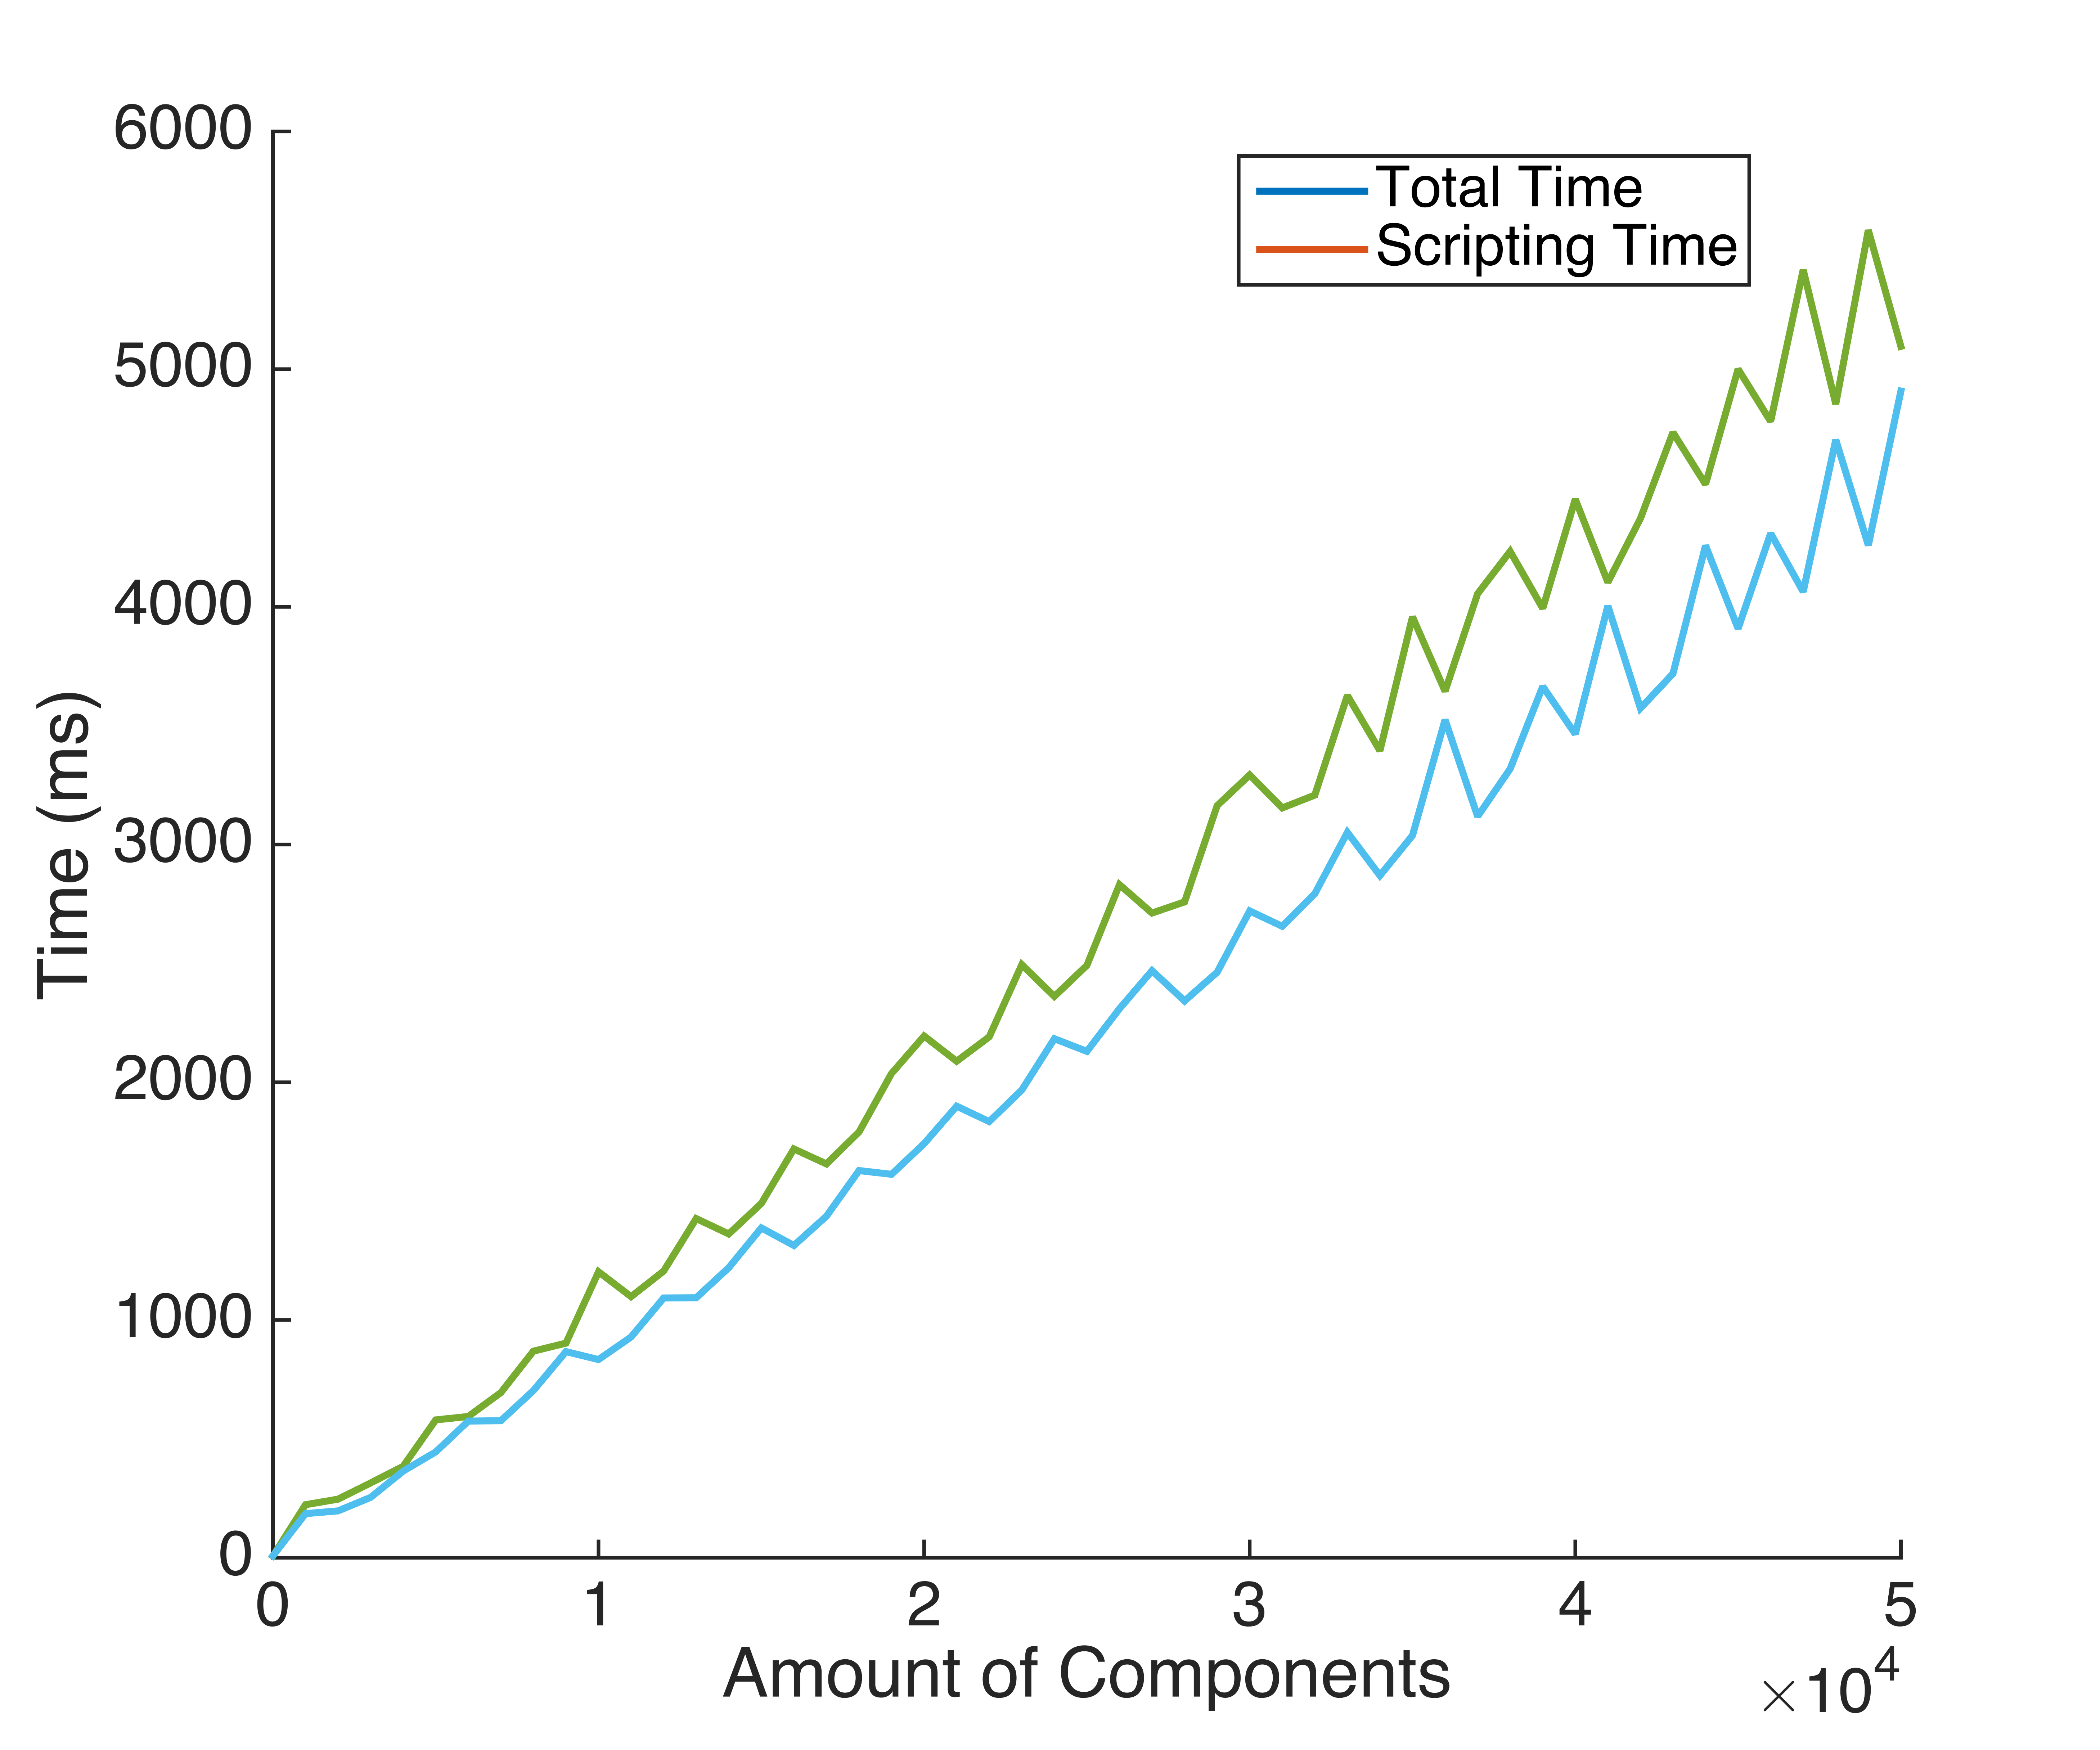
\includegraphics[width=1\textwidth]{Figures/eval-perf.png}
  \caption{Consumption of total time and scripting time in the rendering process of objectified Canvas}
  \label{fig:eval-perf}
\end{figure}

%\subsection{Analysis of Result }

\textbf{Rendering performance is approximately linear to the amount of components}. As shown in the figure \ref{fig:eval-perf}, the total time, which includes scripting time, rendering time and painting time is about 1000 ms when the amount of components is $1\times 10^{4}$. If the amount of Components reaches $5\times 10^{4}$, the total time increases to nearly 5000 ms.

\textbf{Scripting time has accounted for the majority of total time}. As a part of total time, the scripting time , which is also approximately linear, takes the most of time consumption while processing the rendering task. After the objectified Canvas has loaded the image data successfully, it will parse each component defined in the image data and instantiate them as well as add the objects into its own context. However, the actual rendering time, which is the difference of total time and scripting time, is only a fraction in the whole rendering process.

However, the performance test is performed with such a huge range of components' amount, which doesn't represent the usage in normal case. Considering the linearity of the rendering performance, drawing less than 1000 components, which are already huge enough for expressing the graphical content in the real world, will only spend less than 100 ms.